\section{Evaluation}
\label{sec:evaluation}

Two standard metrics are used to measure the accuracy of link mining algorithms: \textit{AUC} and  \textit{Precision} \cite{Lu2011}. We focused here on AUC because it is stronger in revealing false positivity issues.

To apply those metrics, the original dataset is partitioned into a trainset and a testset, according to some given test ratio $\alpha$. \hlm{Formally, for two istants $t$ and $t' > t$, we denote $G[t,t']$ the subgraph of G consisting of all edges with a timestamp between $t$ and $t'$. Identified four times: $t_{0}, t'_{0}, t_{1}, t''_{1}$, with $t_{0}<t'_{0}<t_{1}<t'_{1}$, we refer to $[t_{0},t'_{0}]$ as the \textit{training interval} and $[t_{1},t'_{1}]$ as the \textit{test interval}. For example, applying a \textit{prediction algorithm} on the graph obtained after the training interval, as $G[t_{0},t'_{0}]$, we want to make a prediction on the edges that will be present in the graph $G[t_{1},t'_{1}]$ and not present in $G[t_{0},t'_{0}]$\cite{Liben-Nowell}.}

\hlm{In this work we denote as trainset, and testset, the set of edges of $G$ after the training interval and test interval, respectively. The trainset is obtained removing the $\alpha\%$ of links from the dataset (namely, missing links).}


AUC is defined as follows:
%
\begin{equation}
\label{eqn:auc}
AUC=\frac{n_{1}+0.5n_{2}}{n}
\end{equation}
%
where 
$n_{1}$ is the number of times a missing link has a score greater than an inexistent link,
$n_{2}$ is the number of times a missing link has a score equal to an inexistent link and
$n$ is the total number of combination of missing links and inexistent links.

Our experimental framework consists in measuring the AUC for all metric in Equations~\ref{eqn:common-neighbours}-\ref{eqn:nra-local}, applied to both criminal and not criminal datasets with test ratios $\alpha=10\%$ and $\alpha=15\%$.
%
In particular, we analyze 
(i) a criminal dataset (CRM) collecting wiretrap-records, judgement and arrest warrants \cite{berlusconi2016link}; and
(ii) a business-related dataset (BSN) collecting face-to-face interactions between employees in a IT company \cite{olguin2009sensible}.
%
Notice that, since the evaluated metrics are all local, the considered datasets are all made of a single connected component, so to avoid the distortion in accuracy measurements.

In Table~\ref{tab:auc-detection} and \ref{tab:auc-prediction} we list results for link detection and prediction, respectively, highlighting the most notable ones.
%
The experimental results show that classical metrics achieve great performance in prediction tasks, while the novel metrics do it in detection.
%
In particular, we notice that in prediction some metrics achieve performances clearly distinguishable from others, while in detection they tend to flatten.

\begin{table}[h]
	\centering
	\begin{tabular}{l l l l l}
	\toprule
	\textbf{Metric} & \textbf{CRM-10} & \textbf{CRM-15} & \textbf{BSN-10} & \textbf{BSN-15}\\
	\midrule
		CN   & $68.952$ & $75.227$ & $83.810$ & $75.775$ \\
		SLT  & $66.306$ & $72.919$ & $80.948$ & $73.628$ \\
		JCR  & $66.377$ & $72.981$ & $82.403$ & $75.054$ \\
		SRS  & $66.380$ & $72.985$ & $82.405$ & $75.054$ \\
		HPI  & $66.795$ & $73.507$ & $66.941$ & $63.126$ \\
		HDI  & $66.514$ & $73.064$ & $82.618$ & $75.194$ \\
		LHN1 & $66.100$ & $72.821$ & $59.623$ & $60.386$ \\
		PA   & $80.895$ & $80.383$ & $82.618$ & $75.247$ \\
		AA   & $69.204$ & $76.282$ & $84.351$ & $76.058$ \\
		RA   & $69.156$ & $76.283$ & $84.435$ & $75.875$ \\
		NRA  & $68.784$ & $76.196$ & $71.677$ & $66.472$ \\
		BA   & $69.293$ & $76.477$ & $83.728$ & $75.745$ \\
		NBA  & $68.870$ & $76.277$ & $65.133$ & $65.015$ \\
	\bottomrule
	\end{tabular}
	\caption{AUC for link detection.}
	\label{tab:auc-detection}
\end{table}

\begin{table}[h]
	\centering
	\begin{tabular}{l l l l l}
	\toprule
	\textbf{Metric} & \textbf{CRM-10} & \textbf{CRM-15} & \textbf{BSN-10} & \textbf{BSN-15}\\
	\midrule
		CN   & $82.520$ & $76.970$ & $77.159$ & $75.249$ \\
		SLT  & $80.210$ & $75.150$ & $74.312$ & $70.947$ \\
		JCR  & $80.191$ & $75.208$ & $75.917$ & $73.485$ \\
		SRS  & $80.191$ & $75.208$ & $75.917$ & $73.485$ \\
		HPI  & $81.445$ & $76.001$ & $63.194$ & $60.791$ \\
		HDI  & $80.210$ & $75.223$ & $75.788$ & $73.631$ \\
		LHN1 & $79.890$ & $75.028$ & $59.333$ & $57.635$ \\
		PA   & $83.314$ & $81.655$ & $74.987$ & $74.373$ \\
		AA   & $81.745$ & $77.593$ & $76.770$ & $75.149$ \\
		RA   & $81.702$ & $77.497$ & $76.023$ & $74.697$ \\
		NRA  & $81.322$ & $77.363$ & $61.993$ & $63.661$ \\
		BA   & $82.292$ & $77.769$ & $73.044$ & $72.116$ \\
		NBA  & $81.781$ & $77.581$ & $63.457$ & $63.364$ \\
	\bottomrule
	\end{tabular}
	\caption{AUC for link prediction.}
	\label{tab:auc-prediction}
\end{table}	

\hlm{MANCA COMMENTO DETTAGLIATO SUI RISULTATI OTTENUTI}.

% OLD
%Formally, for two istants $t$ and $t' > t$, we denote $G[t,t']$ the subgraph of G consisting of all edges with a timestamp between $t$ and $t'$. Identified four times: $t_{0}, t'_{0}, t_{1}, t''_{1}$, with $t_{0}<t'_{0}<t_{1}<t'_{1}$, we refer to $[t_{0},t'_{0}]$ as the \textit{training interval} and $[t_{1},t'_{1}]$ as the \textit{test interval}. Applying a \textit{prediction algorithm} on the graph obtained after the training interval, as $G[t_{0},t'_{0}]$, we want to make a prediction on the edges that will be present in the graph $G[t_{1},t'_{1}]$ and not present in $G[t_{0},t'_{0}]$\cite{Liben-Nowell}.
%In this work, the notions of training interval and test interval, are provided with the only purpose to test the algorithm that will be presented in the following. After all, this application produce an output of links mining in real time: in which each instant $t\textsuperscript{*}>t_{0}$ identifies a graph $G[t_{0},t\textsuperscript{*}]$ on which to execute the algorithm. More details about the real time processing are explained in Section \ref{sec:architecture}.

%Notice that, in this work we assume that the graph is connected, therefore each pair of nodes is connected by a path. If we had in the case of a not connected graph, with a large connected component, as \textit{giant component}, and other small size connected components, the accuracy would be distorted by different \textit{density} of edges in a connected components.

%\begin{figure}
%	\centering
%	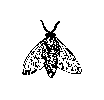
\includegraphics{./fig/fly}
%	\caption{AUC and Precision indices for link detection metric, considering both a criminal and a social network dataset.}
%	\label{fig:performance-detection}
%\end{figure}

%\begin{figure}
%	\centering
%	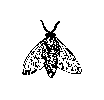
\includegraphics{./fig/fly}
%	\caption{AUC and Precision indices for link prediction metric, considering both a criminal and a social network dataset.}
%	\label{fig:performance-prediction}
%\end{figure}
